\section{Neural Machine Translation}
\subsection{Word Vector Semantics and Word Embeddings}
We make the \textbf{distributional hypothesis}: the \emph{meaning} of a word is \emph{its use} in the language.
Language use can thus be characterized by \emph{counting} how many often \emph{other words occur} in the context of appearance of a specific word.

\emph{Co-occurrence frequencies} between a target word and other context words can be stored in a vector representing the target word meaning\footnote{We thus use the following notation: \(v\) is a word, and \(\bm{v}\) is a vector representing it.}.
The \emph{context} can be a \emph{document}, \emph{paragraph}, \emph{sentence} or a \emph{local context} before and after the target word.
This information can be stored in a \emph{co-occurrence matrix}, where each \emph{row} defines the \emph{vector} associated to a specific word, and the number of \emph{columns} depends on the number of contextual words, which is by default the whole vocabulary for the task.

The \emph{similarity between word meanings} can thus be \emph{computed} from the \emph{vector similarity} in \(\R^d\), with \(d\) approximately the vocabulary size.
Typically, the \emph{cosine similarity} is used:
\[
\cos(\bm{v}, \bm{w}) = \frac{\langle \bm{v}, \bm{w}\rangle}{\norm{\bm{v}}\norm{\bm{w}}} = \frac{\sum_{i = 1}^d v_i w_i}{\sqrt{\sum_{i=1}^d v_i^2} \sqrt{\sum_{i=1}^d w_i^2}}.
\]
This value is maximal (equal to \(1\)) when the angle between \(\bm{v}\) and \(\bm{w}\) is \(0\), which means the \emph{relative frequencies} of \emph{all} co-occurring words are \emph{the same}.

Actual \textbf{vector semantics} are based on \emph{weighted} and \emph{normalized frequencies}, because raw counts are \emph{very skewed} and not very \emph{discriminative}, as there is a lot of co-occurrence with non-informative function words.
Several strategies exist to mitigate this problem.
Note that such methods define \emph{sparse word embeddings}, meaning there are a lot of zeros in the co-occurrence matrix.
The solution is to use a vector space of \emph{smaller dimensionality} instead of the vocabulary size, using fewer parameters to represent word meanings.
Rather than defining word embeddings from (weighted) co-occurrence counts, we \emph{learn dense word embeddings}: this also means that the dimensions of the vector space no longer represent co-occurring words, but are \emph{abstract dimensions} which are \emph{automatically defined by a learning algorithm}.
Word embeddings are learned to \emph{solve a specific NLP task}, such as \emph{sentiment analysis}, \emph{sentence completion}, or can be reused for tasks like \emph{translation}.
Learned embeddings are typically \emph{dense}.

One such embedding is \textbf{Word2Vec}.
It follows the following general scheme:
\begin{enumerate}
	\item Learn skip-grams embedding to solve a \emph{binary prediction task}: is a word \(w\) particularly likely to occur in a context of the target word \(t\)?
	For this, treat words and neighboring context words (skip-bigrams) as \emph{positive examples}, and randomly sample other words from the vocabulary to form \emph{negative examples}.
	\item Train a \emph{logistic regression} as a classifier to discriminate positive and negative examples.
	\item Use \emph{regression weights} as word embeddings.
\end{enumerate}

Given a target word \(t\) and a candidate context word \(c\), define the \emph{probability} \(\Pr(+ \mid t, c)\) that \(c\) is a positive example.
\(\Pr(+ \mid \bm{t}, \bm{c})\) is a function of the vectors \(\bm{t}\) and \(c\) representing \(t\) and \(c\).
Note that \(\langle \bm{t}, \bm{c} \rangle\) measures the \emph{similarity} between \(t\) and \(c\) (it corresponds to an unscaled cosine similarity).
This measure is \emph{squashed} between \(0\) and \(1\) by a \emph{sigmoid/logistic function}:
\[
\Pr(+ \mid \bm{t}, \bm{c}) = \sigma(\langle \bm{t}, \bm{c}\rangle), \quad \textnormal{where} \quad \sigma(x) = \frac{1}{1 + e^{-x}} = \frac{e^x}{e^x + 1}.
\]
Note that \(\Pr(- \mid \bm{t}, \bm{c}) = 1 - \Pr(+ \mid \bm{t}, \bm{c})\).
The learning algorithm starts with \emph{randomly chosen vectors} in \(d\) dimensions, where \(d\) is a fixed hyperparameter.
These vectors are then \emph{greedily optimized} to better fit the training data.

More formally, let \(\theta\) be the set of model parameters, i.e. vectors \(\bm{t}\) and \(\bm{c}\) for all target/context words.
We then define the \emph{log-lokelihood}
\[
\mathrm{LL}(\theta) = \sum_{t, c \in +} \log \Pr(+ \mid \bm{t}, \bm{c}) + \sum_{t, c \in -} \log \Pr(- \mid \bm{t}, \bm{c}),
\]
which measures the fit to the positive and training examples.
We want to \emph{increase} the similarity between real context words, and \emph{decrease} it for random noise words.
Our optimization goal is to find the parameters \(\theta\) that maximize \(\mathrm{LL}(\theta)\), or equivalently, minimize \(-\mathrm{LL}(\theta)\), which we call the \emph{negative log-likelihood loss}.
The standard technique for this is \emph{gradient descent}.
The final result of this learning algorithm is a set of \(d\)-dimensional embeddings for \(T\) and \(C\), the sets of target words and context words.
The choice then needs to be made to either just keep \(T\), to add them element-wise, or to concatenate them, turning it into a \(2d\)-dimensional embedding.

Popular word embeddings such as Word2Vec or GloVe are effective ways to represent \emph{word meanings} by \emph{vectors}.
Notably, \emph{vector arithmetic} allows us to \emph{combine meanings}, but word embeddings include \emph{gender} or \emph{racist} biases, most likely present in the corpora they are trained from.

\subsection{Brief Introduction to Deep Learning}
Recent advances in ML, and particularly, \emph{deep learning} (which refers to a family of ML methods relying on \emph{neural networks} including many layers), have allowed to outperform phrase-based models.

To introduce DL, we assume a problem of binary classification, where we must assign \(\pm 1\) to a vector \(\bm{x}\).
For this, we use a \emph{linear model}:
\[
f(\bm{x}) = \mathrm{sign}\left(\sum_{i = 1}^d w_i x_i + w_0\right).
\]
This model defines a \emph{hyperplane} (a \emph{linear decision boundary}) in a \(d\)-dimensional space.
The vector \(\bm{w}\) represents the orientation of the hyperplane, whereas \(w_0\) is its shift w.r.t. the origin.
These are the \emph{model parameters}, to be estimated from a learning sample.

The simplest network representing a linear classifier is the \textbf{perceptron}, shown in Figure~\ref{fig:perceptron}.
\begin{figure}[!hbtp]
	\centering
	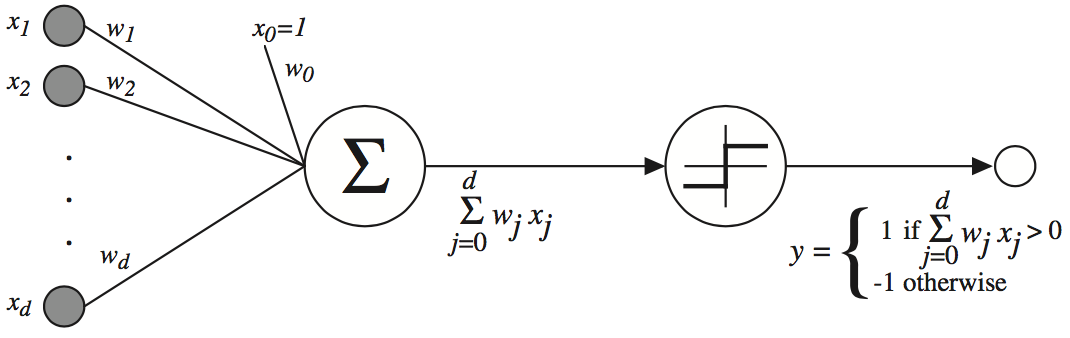
\includegraphics[width=\textwidth]{img/perceptron}
	\caption{Perceptron}
	\label{fig:perceptron}
\end{figure}
It contains the following elements:
\begin{itemize}
	\item the \emph{input layer} is made out of \emph{neurons}, each one excited at the corresponding \(x_j\) value;
	\item the \emph{weight vector} \(\bm{w}\) is associated to \emph{synapses}, which are weighted links between neurons;
	\item the \emph{output} \(y = f(\bm{x})\) is computed after going through an \emph{activation function}, here the \emph{sign} function corresponding to a thresholding function; in practice, this is often replaced by a continuous and \emph{differentiable} approximation such as \(\tanh\).
\end{itemize}

To learn the parameters of the perceptron model, \emph{gradient descent} is used:
\begin{enumerate}
	\item Initialize \(\bm{w}\) to small random values.
	\item \label{gds2}Compute the predicted output \(\hat{y}_i\) for each sample \(i\) in the training set.
	\item Compute the \emph{loss function} \(L(\hat{\bm{y}}, \bm{y})\) measuring the discrepancy between the predicted \(\hat{\bm{y}}\) and the target values \(\bm{y}\), defined by the labeling (\(\pm 1\)) of the learning examples.
	A possible loss is the \emph{square loss}:
	\[
	L(\hat{\bm{y}}, \bm{y}) = \frac{1}{2}\sum_{i} (\hat{y}_i - y_i)^2.
	\]
	\item \label{gds4}\emph{Update the weight vector} to reduce the loss by \emph{gradient descent}:
	\[
	\bm{w} \gets \bm{w} - \eta \nabla_{\bm{w}} L(\hat{\bm{y}}, \bm{y}),
	\]
	where \(\eta\) is a learning rate hyperparameter.
	\item Iterate steps \ref{gds2} through \ref{gds4} until convergence.
\end{enumerate}

The perceptron can be generalized by adding one or several \emph{hidden layers}, and possibly, \emph{multiple outputs}.
This is called a \textbf{multi-layer perceptron} (MLP).
MLPs can be learnt using the \emph{back-propagation algorithm}, which generalizes gradient descent by applying the \emph{chain rule} of derivatives.
MLPs can represent arbitrary \emph{non-linear functions} (under certain technical conditions).
Note that each hidden layer \(\bm{h}\) can be seen as a \emph{novel representation} of the data, which is automatically learnt, once the network topology is fixed.
In particular, when the inputs are words, the first layer defines a \emph{word embedding}.
Stacking up many such layers leads to a \emph{deep feedforward network}.

\subsection{Deep Learning Methods for Sequential Data}
Textual input can be represented using a \emph{one-hot encoding}.
Let \(\mathbf{Voc}\) be a set of words representing the \emph{vocabulary}.
Each \emph{word} can then be represented as a \emph{variable-length sequence of vectors} \(\bm{x}_1, \bm{x}_2, \dots, \bm{x}_t, \dots\), each with a single nonzero element set to \(1\).
\emph{Machine translation} maps an \emph{input/source vector sequence} \(\bm{x}_1, \dots, \bm{x}_M\) to an \emph{output/target vector sequence} \(\bm{y}_1, \dots, \bm{y}_N\).

We can then build the following neural language model, shown in Figure~\ref{fig:neural_language_model}.
\begin{figure}[!hbtp]
	\centering
	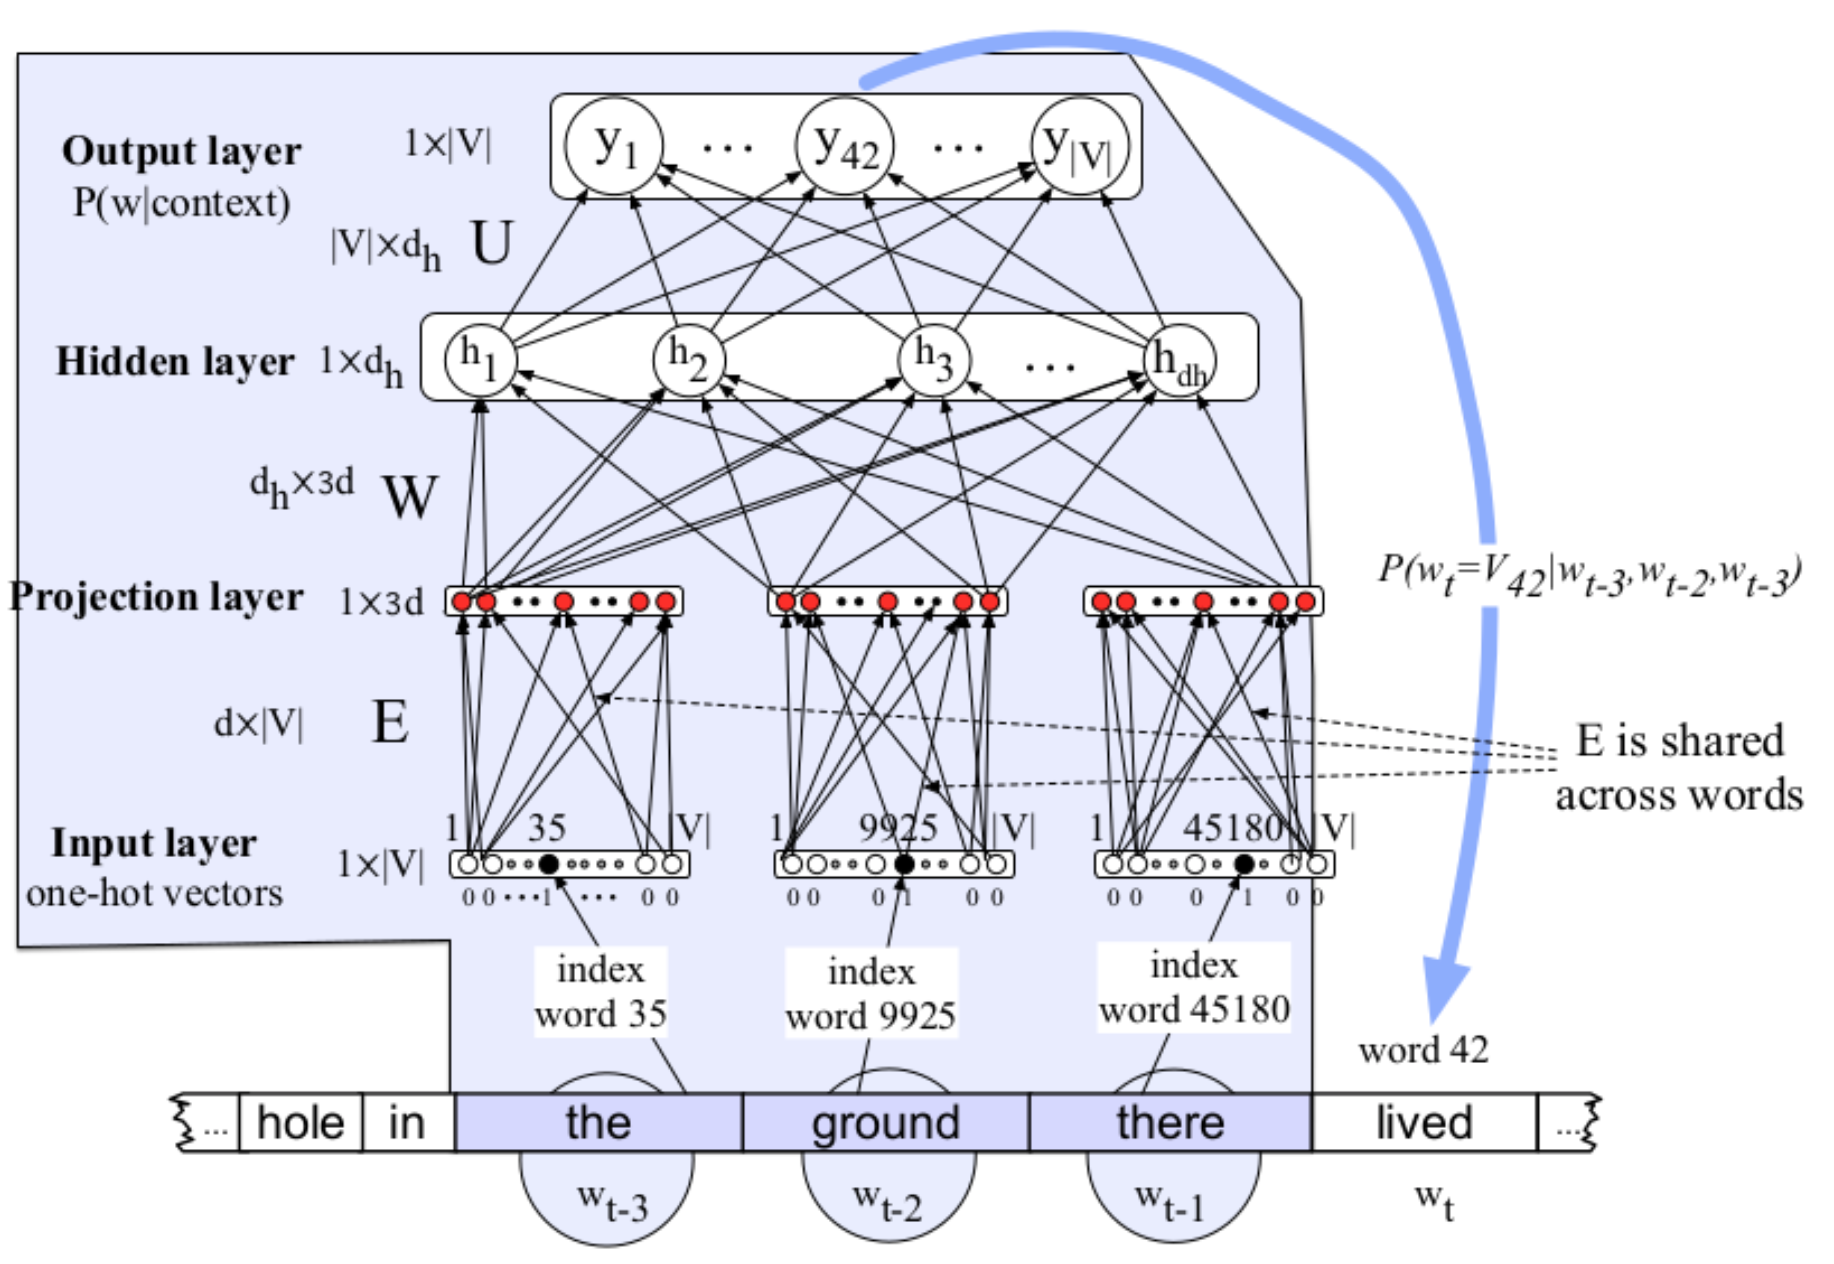
\includegraphics[width=\textwidth]{img/neural_language_model}
	\caption{\emph{Feedforward network} implementing a \(4\)-gram}
	\label{fig:neural_language_model}
\end{figure}
This network works as follows:
\begin{itemize}
	\item The \emph{output (softmax) layer} (a sigmoid generalization), which computes
	\[
	\Prhat(w_t = i \mid w_{t_3} w_{t_2} w_{t-1}) = \mathrm{softmax}(y_i) = \frac{\exp(y_i)}{\sum_{i' = 1}^{\abs{\mathbf{Voc}}} \exp(y_{i'})}.
	\]
	\item The \emph{first layer} computes a \emph{word embedding}, possibly initialized from a pre-trained model, and re-estimated jointly when learning the network weights.
	\item The network is trained to minimize the \emph{negative log-likelihood loss} (or perplexity):
	\[
	-\sum_{t = 1}^M \log \Prhat(w_t \mid w_{t-3} w_{t-2} w_{t-1}),
	\]
	with \(M\) the number of training tokens.
\end{itemize}
Note that the \emph{network topology} depends on the model order, and ignores any longer (left-)contexts.

To deal with sequential data of arbitrary length, we introduce \emph{recurrent neural networks}, as shown schematically on Figure~\ref{fig:rnn}.
\begin{figure}[!hbtp]
	\centering
	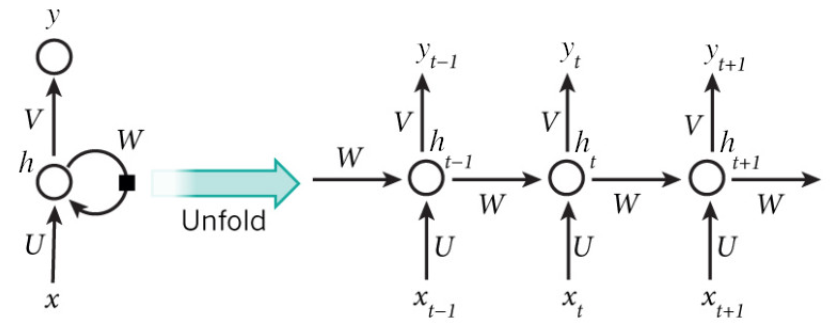
\includegraphics[width=\textwidth]{img/rnn}
	\caption{Recurrent neural network}
	\label{fig:rnn}
\end{figure}
RNNs are governed by the system
\[
\left\{\begin{array}{rcl}
\bm{h}_t & = & \tanh(U\bm{x}_t + W\bm{h}_{t-1}),\\
\bm{y}_t & = & V \bm{h}_t,
\end{array}\right.
\]
where \(\bm{h}_{t-1}\) represents the \emph{state} at the \emph{previous step} (\(t-1\)) and is combined with \(\bm{x}_t\) to predict the \emph{current state} \(\bm{h}_t\).
RNN weights (\(U, V, W\)) can be learnt by unfolding the recurrence in time.
This is called \emph{back-propagation through time} (BPTT).
The \emph{same weights} are used at each time step, but \((\bm{x}_t, \bm{h}_t, \bm{y}_t)\) evolve.

RNNs can be used to perform several NLP tasks, such as \emph{sentence generation} and \emph{POS tagging}.
As they have no fixed size context, but a recurrence, they can in principle capture \emph{arbitrarily long term dependencies}.
As with other NNs, RNNs can be \emph{stacked} to learn and to represent \emph{progressive abstractions} of the input data.
\emph{Bi-directional RNNs} combine \emph{left} and \emph{right context}, which can be useful for e.g. POS tagging.

\subsection{Deep Networks for Machine Translation}
\textbf{Machine translation} is similar to \emph{POS tagging} as it maps an input sequence to an output sequence.
However,
\begin{itemize}
	\item Unlike POS tagging, machine translation is \emph{not a one-to-one mapping}: the \emph{input length} may differ from the \emph{output length}, and \emph{word re-ordering occurs}.
	This can be solved with encoder-decoder networks.
	\item BPTT has a hard time converging for \emph{long term dependencies}, which are prevalent in translation.
	This is because of the \emph{vanishing/exploding} gradients.
	This problem is solved with LSTM networks.
\end{itemize}

\subsubsection{Long Short-Term Memory}
The \textbf{LSTM} cell, shown on Figure~\ref{fig:lstm}, is governed by the following equations:
\begin{align*}
	\bm{i}_t &= \sigma(W_{xi} \bm{x}_t + W_{hi} \bm{h}_{t-1} + W_{ci} \bm{c}_{t-1}),\\
	\bm{o}_t &= \sigma(W_{xo} \bm{x}_t + W_{ho} \bm{h}_{t-1} + W_{co} \bm{c}_{t-1}),\\
	\bm{f}_t &= \sigma(W_{xf} \bm{x}_t + W_{hf} \bm{h}_{t-1} + W_{cf} \bm{c}_{t-1}),\\
	\bm{c}_t &= \bm{f}_t \cdot \bm{c}_{t-1} + \bm{i}_t \tanh(W_{xc} \bm{x}_t + W_{hc} \bm{h}_{t_1}),\\
	\bm{h}_t &= \bm{o}_t \tanh(\bm{c}_t).
\end{align*}
Note that cell state \(\bm{c}_t\) depends on \(\bm{x}_t\) and \(\bm{c}_{t-1}\) (as in a standard RNN) to produce \(\bm{h}_t\) (such ``output'' becomes ``hidden'' when being the ``input'' to the next layer).
\begin{figure}[!hbtp]
	\centering
	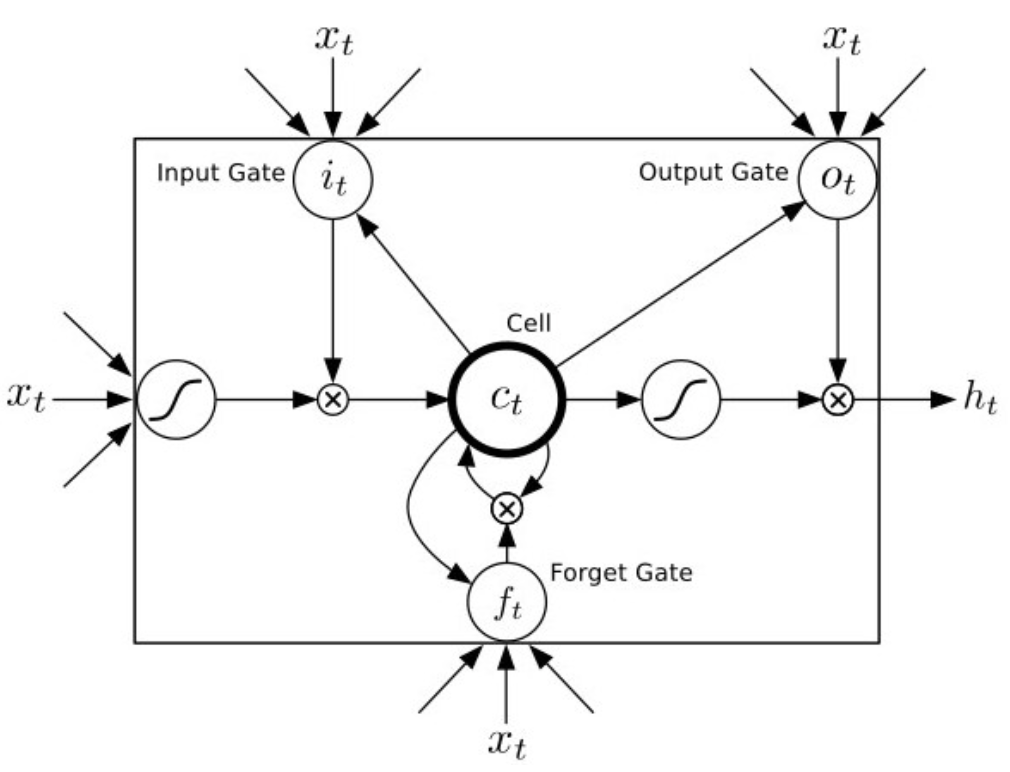
\includegraphics[width=0.7\textwidth]{img/lstm}
	\caption{Long short-term memory cell}
	\label{fig:lstm}
\end{figure}
The \emph{LSTM memory cell} is controlled by 3 \emph{multiplicative gates}:
\begin{itemize}
	\item the \emph{input gate} is a switch to transmit \(\bm{x}_t\);
	\item the \emph{output gate} controls whether \(\bm{h}_t\) depends on \(\bm{c}_t\); and
	\item the \emph{forget gate} controls whether \(\bm{c}_t\) depends on \(\bm{c}_{t-1}\).
\end{itemize}
All weights (including those controlling the gates) can be learnt with BPTT.
We thus have a \emph{short-term dependency} thanks to \(\bm{c}_{t-1}\) and a \emph{long-term memory} thanks to the \emph{weights}.

This idea can be adapted to take into account past (left) and future (right) context, called a \emph{bidirectional LSTM}, shown on Figure~\ref{fig:bilstm}.
\begin{figure}[!hbtp]
	\centering
	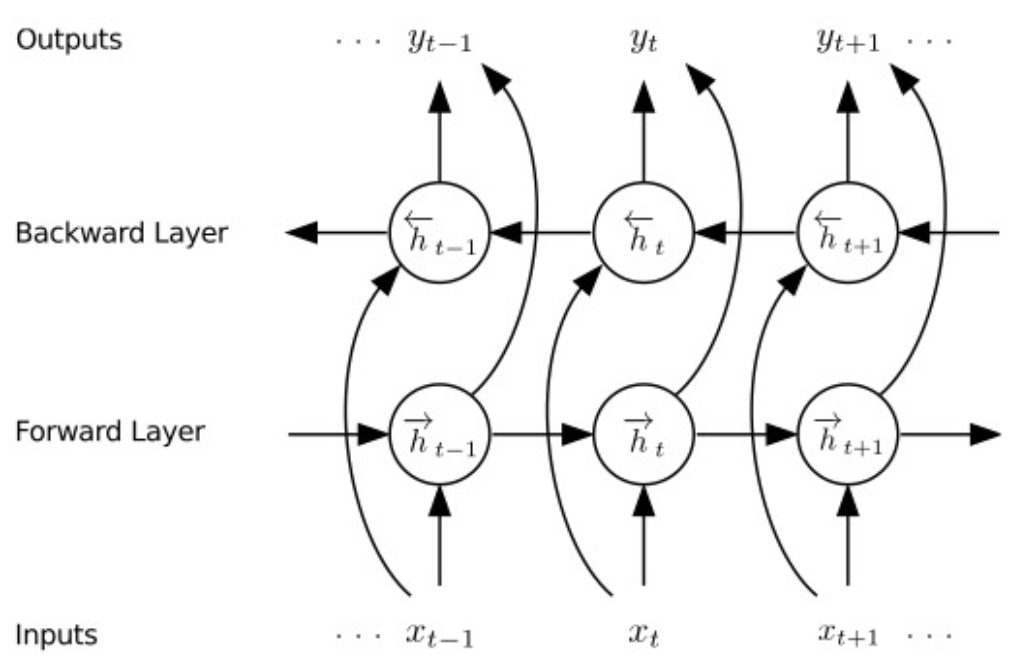
\includegraphics[width=0.7\textwidth]{img/bilstm}
	\caption{Bidirectional LSTM}
	\label{fig:bilstm}
\end{figure}
Is is governed by the following equations:
\begin{align*}
	\overrightarrow{\bm{h}}_t &= \mathscr{H}\left(W_{x\overrightarrow{h}} \bm{x}_t + W_{\overrightarrow{h}\overrightarrow{h}} \overrightarrow{\bm{h}}_{t-1}\right)\\
	\overleftarrow{\bm{h}}_t &= \mathscr{H}\left(W_{x\overleftarrow{h}} \bm{x}_t + W_{\overleftarrow{h}\overleftarrow{h}} \overleftarrow{\bm{h}}_{t+1}\right)\\
	\bm{y}_t &= W_{\overrightarrow{h} y} \overrightarrow{\bm{h}}_t + W_{\overleftarrow{h} y} \overleftarrow{\bm{h}}_t,
\end{align*}
where \(\mathscr{H}\) represents the nonlinearities within an LSTM cell.
The \emph{forward layer} processes the input from left to right, whereas the \emph{backward layer} processes the input from right to left.
The output \(\bm{y}_t\) is a weighted sum of both.

\subsubsection{Encoder-Decoder Structure}
The \textbf{encoder-decoder structure}, is shown on Figure~\ref{fig:encdec}.
\begin{figure}[!hbtp]
	\centering
	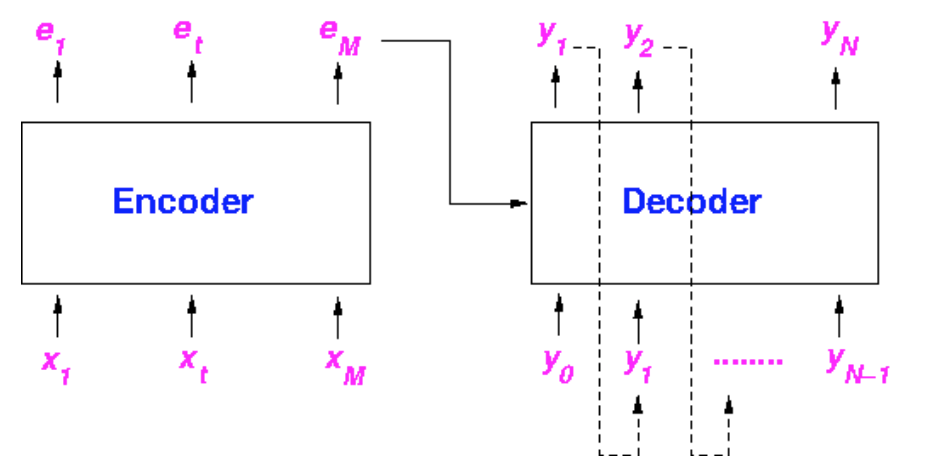
\includegraphics[width=0.7\textwidth]{img/encdec}
	\caption{Encoder-decoder structure}
	\label{fig:encdec}
\end{figure}
The \emph{encoder}, implemented as e.g. stacked bidirectional LSTMs, gradually encodes the input in another sequence.
The \emph{last deep representation} \(\bm{e}_M = (\bm{h}_M, \bm{c}_M)\) of the input sequence is passed to the \emph{decoder}:
\begin{itemize}
	\item \(\bm{h}_M\) is the output of the last level when \(\bm{x}_M\) is fed as input, and
	\item \(\bm{c}_M\) is the cell state of the last level when \(\bm{x}_M\) is fed as input.
\end{itemize}
The \emph{decoder} generates the output sequence from \(\bm{e}_M\) and the predicted \(\bm{y}_{i-1}\), with \(\bm{y}_0\) the one-hot encoding of \stoken.

In its simplest form, the computation can be formulated using the \emph{conditional probability of the translation} to produce a sequence \(Y\) from a sequence \(X\):
\begin{align*}
	\Pr(Y \mid X) &= \Pr(Y \mid \bm{x}_1, \dots, \bm{x}_M)\\
	&= \prod_{i=1}^N \Pr(\bm{y}_i \mid \bm{y}_0, \dots, \bm{y}_{i-1}, \bm{x}_1, \dots, \bm{x}_M)\\
	&\approx \prod_{i=1}^N \Pr(\bm{y}_i \mid \bm{y}_0, \dots, \bm{y}_{i-1}, \bm{e}_M).\\
\end{align*}
This can be extended with \emph{attention modules}, which consider the whole sequence \(\bm{e}_1, \dots, \bm{e}_M\) instead of just \(\bm{e}_M\).

\subsubsection{Google Translate Architecture}
The \textbf{Google Translate architecture} shown in Figure~\ref{fig:google_translate} combines these previous ideas:
\begin{itemize}
	\item 1 bidirectional LSTM layer + 7 LSTM layers \emph{encode} the input \(\bm{x}_1, \dots, \bm{x}_t, \dots, \bm{x}_M\) into a \emph{deep representation} for each time step \(\bm{e}_1, \dots, \bm{e}_t, \dots, \bm{e}_M\).
	\item 8 LSTM layers \emph{decode} it to produce an output vector sequence \(\bm{y}_1, \dots, \bm{y}_i, \dots, \bm{y}_N\).
	\item An \emph{attention module} links the \emph{encoder} and \emph{decoder}.
	\item The word \(w_i\) output at step \(i\) is computed through a \emph{softmax} layer:
	\[
	\Pr(w_i = \textnormal{word}^j \mid \bm{x}_1, \dots, \bm{x}_t, \dots, \bm{x}_M) = \frac{\exp[(\bm{y}_i)_j]}{\sum_{j'} \exp[(\bm{y}_i)_{j'}},
	\]
	and \(\bm{y}_i\) is the output of the last layer.
\end{itemize}
\begin{figure}[!hbtp]
	\centering
	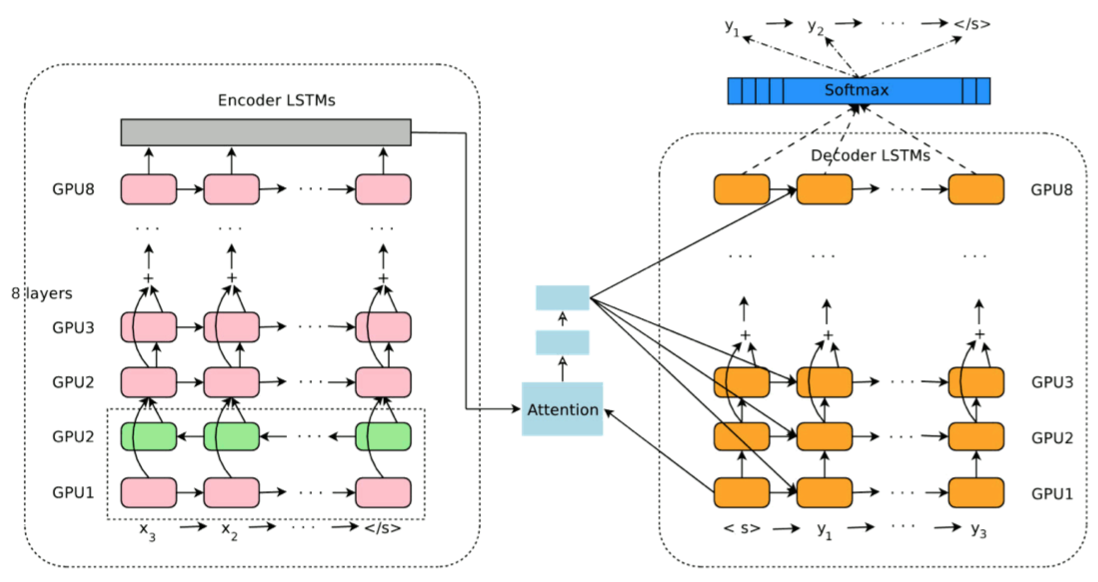
\includegraphics[width=\textwidth]{img/google_translate}
	\caption{Google Translate architecture}
	\label{fig:google_translate}
\end{figure}

The attention mechanism is governed by the following equations:
\begin{align*}
	s_t &= \mathrm{attention}(\bm{h}_{i-1}^\textnormal{dec}, \bm{e}_t),\\
	p_t &= \frac{\exp(s_t)}{\sum_{t' = 1}^M \exp(s_{t'})},\\
	\bm{a}_i &= \sum_{t'=1}^M p_{t'} \cdot \bm{e}_{t'},
\end{align*}
where
\begin{itemize}
	\item The attention function is implemented as a \emph{one layer feedforward network}.
	\item \(\bm{e}_t = (\bm{h}_t, \bm{c}_t)\) are the \emph{encoder output} and \emph{last cell state} at step \(t\) of the input.
	\item \(\bm{h}_{i-1}^\textnormal{dec}\) is measured at the \emph{output} of the \emph{first decoder layer}.
	\item \(\bm{a}_i\) is a \emph{position-dependent weighted sum} fed to the decoder.
\end{itemize}

In this formulation, called \emph{max probability decoding}, we compute \(w_i = \argmax_j \Pr(w_i = \textnormal{word}^j \mid \bm{x}_1, \dots, \bm{x}_M)\), and we use one-hot encoding of \(w_i\) to produce \(\bm{y}_i\) as next input to the decoder.
Decoding stops when the most likely predicted token is \etoken.
In \emph{beam search}, we consider the top-\(k\) outputs at each step and keep the best scored alternatives.
The Google implementation includes a \emph{length normalization} of the alternative scores, and a \emph{coverage penalty} to favor translations that better cover the source sentence according to the attention module.